\section{Qwen-2.5-Math}

\subsection{横向对比其他模型的得分表现}

\begin{frame}{横向对比其他模型的得分表现}
	\begin{figure}[htbp]
		\centering
		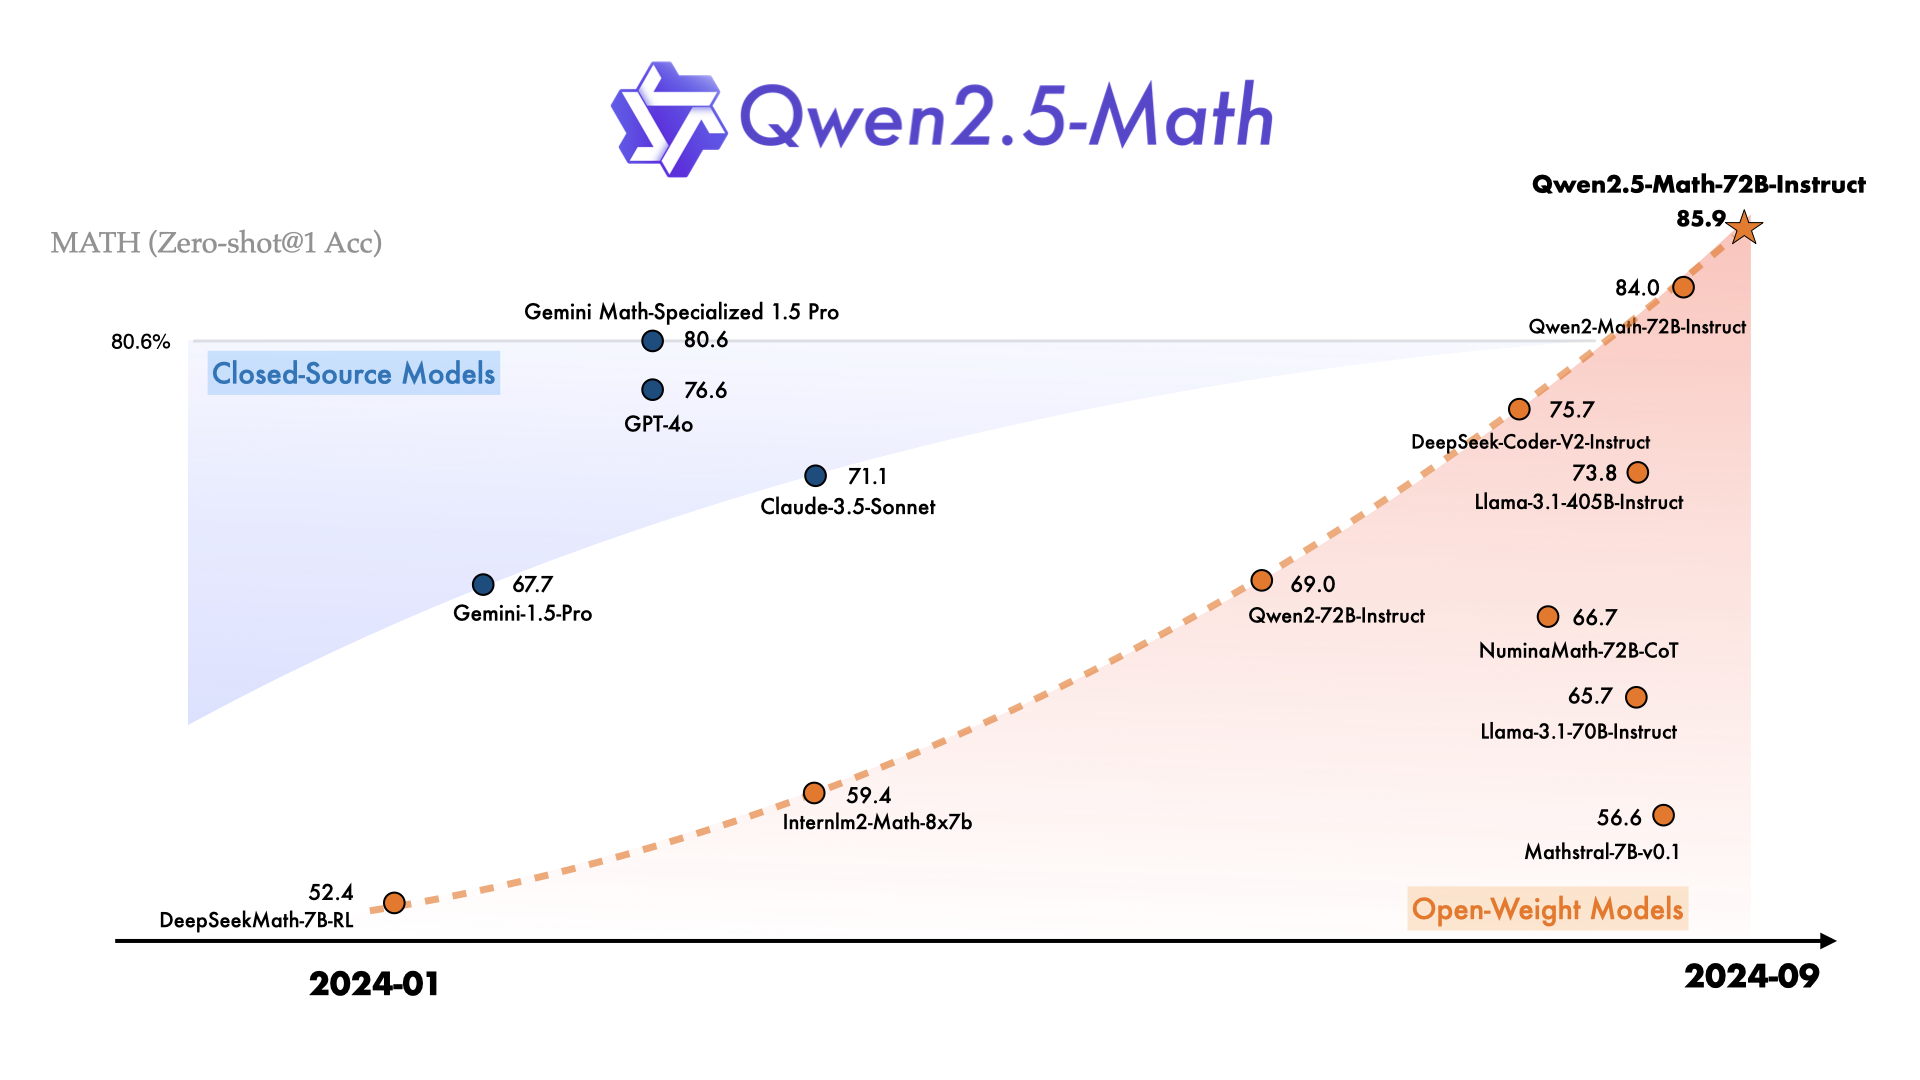
\includegraphics[width=0.7\textwidth]{pic/flagship.png}
		% \vspace{-1mm}
		\caption{The pass@1 performance of Qwen2.5-Math-72B-Instruct on MATH by the Chain-of-Thought reasoning.}
		\label{fig:intro}
	\end{figure}
\end{frame}

\subsection{Self-improvement techniques}
\begin{frame}{Self-improvement techniques}
	\begin{itemize}
		\item In pre-training, we employ Qwen2-Math-Instruct to synthesize math queries and corresponding responses on a large scale to enrich the pre-training corpus of Qwen2.5-Math.\\[0.2cm]
		      \pause
		\item In post-training, we train a reward model on massive sampling from previous models and apply it to the iterative evolution of data in supervised fine-tuning.\\[0.2cm]
		      \pause
		\item Use Qwen2.5-Math-RM in reinforcement learning and best-of-N sampling during inference.
	\end{itemize}

\end{frame}

\subsection{Qwen 2.5 math 的训练流程}
\begin{frame}{Qwen 2.5 math 的训练流程}\small
	\begin{columns}
		\begin{column}{0.6\textwidth}
			\begin{figure}[htbp]
				\centering
				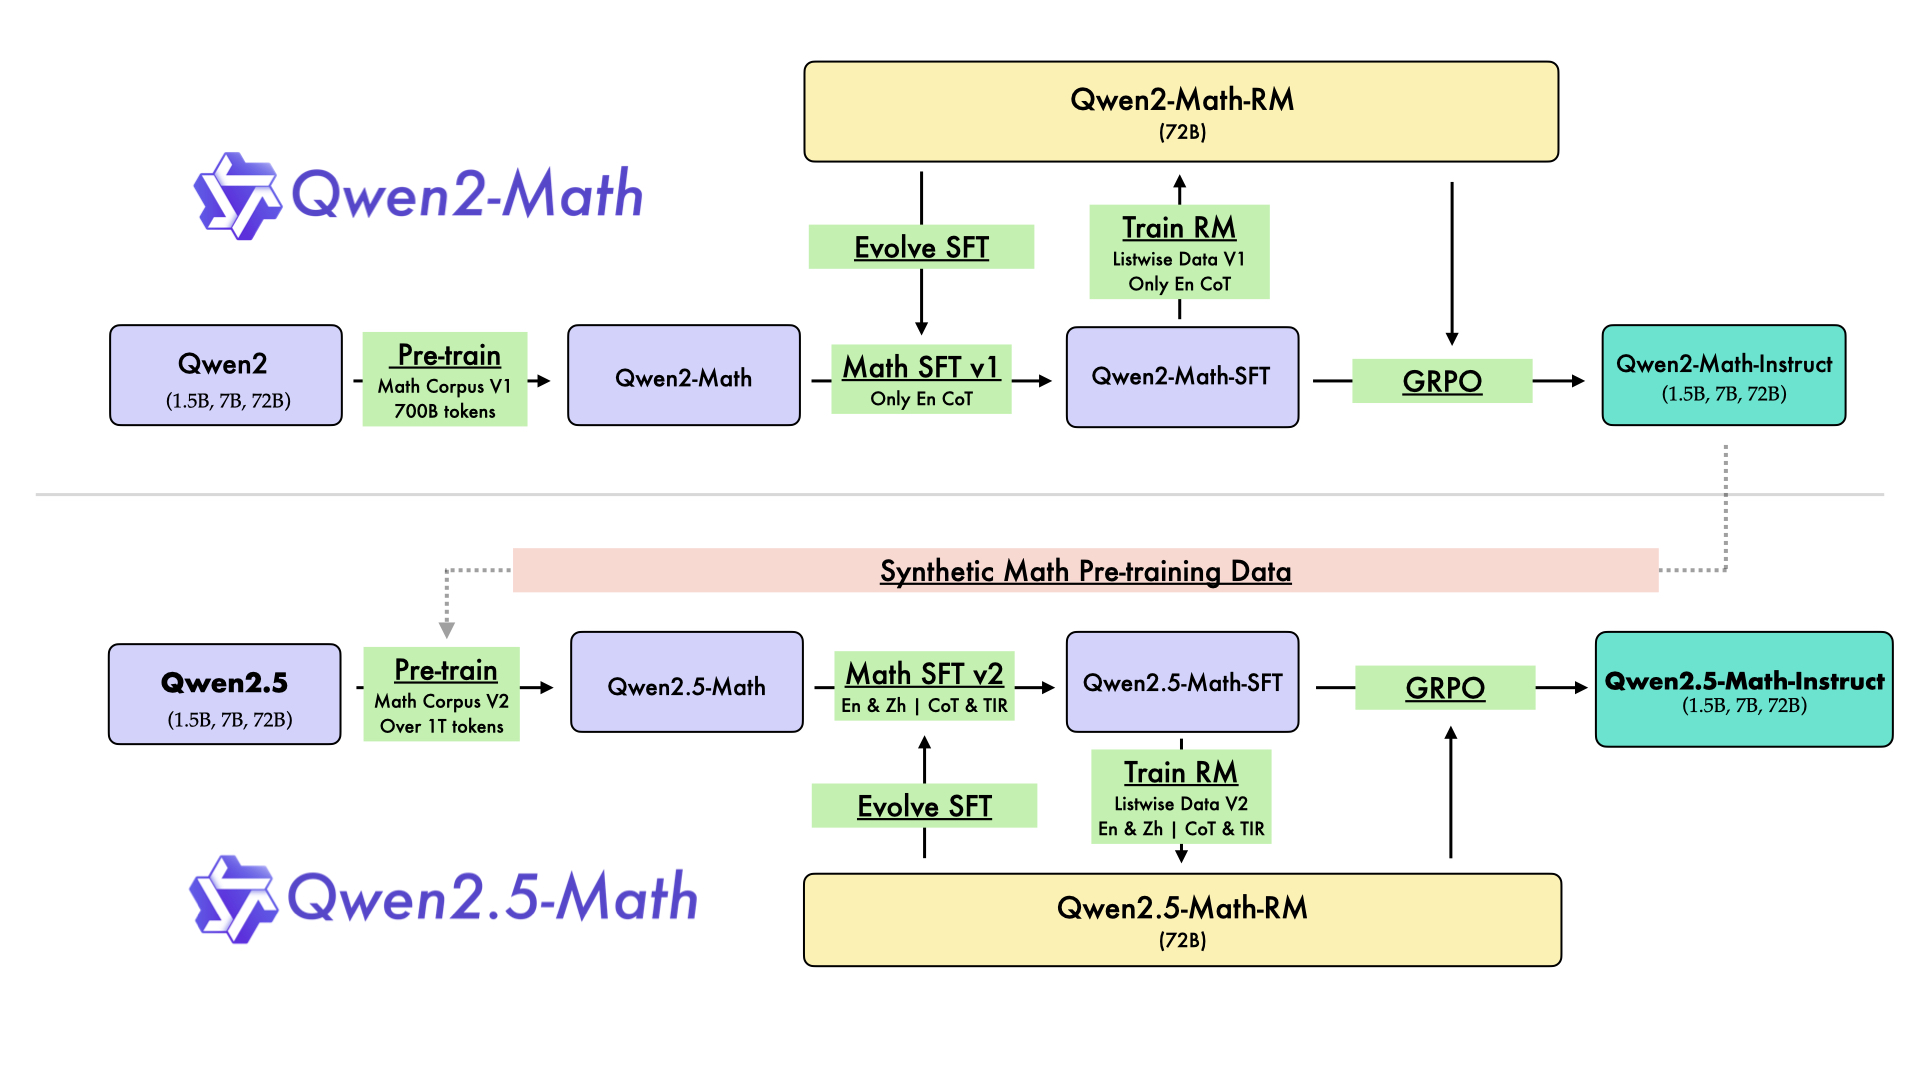
\includegraphics[width=1\columnwidth]{pic/qwen2.5-math-pipeline.jpeg}
				\vspace{-1mm}
				\caption{The development pipelines of Qwen2-Math and Qwen2.5-Math. }
				\label{fig:pipeline}
			\end{figure}
		\end{column}

		\begin{column}{0.4\textwidth}
			\begin{enumerate}
				\item Start -> Qwen Math Corpus v1 (700B tokens) -> Qwen2-Math Base Models
				\item Qwen2-Math-72B -> Qwen2-Math-RM -> SFT Data -> Qwen2-Math-Instruct
				\item Qwen2-Math-72B-Instruct -> Additional Data -> Qwen Math Corpus v2 (1T tokens)
				\item Qwen Math Corpus v2 -> Qwen2.5-Math Models
				\item Qwen2.5-Math-RM -> Qwen2.5-Math-Instruct
			\end{enumerate}
		\end{column}
	\end{columns}
\end{frame}

\subsection{pre-training}
\begin{frame}{data}
	quantity:
	\begin{enumerate}
		\item Train a FastText classifier utilizing high-quality mathematical seed data and general text data.
		      \pause
		\item Leverage meta-information from the recalled data to expand the data pool for mathematical data retrieval.
		      \pause
	\end{enumerate}
	quality:
	\begin{enumerate}
		\item Utilize the Qwen2-0.5B-Instruct model, augmented with prompt engineering, to evaluate the quality of potential data entries.
		      \pause
		\item Employ the Qwen2-72B-Instruct model to synthesize a large amount of mathematical pre-training corpus.
	\end{enumerate}
\end{frame}

\subsection{post-training}
\begin{frame}{post-training}
	\begin{itemize}
		\item Aggregate more high-quality mathematical data, especially in Chinese, sourced from web documents, books, and code repositories across multiple recall cycles. Qwen Math Corpus v1(700B tokens) -- >Qwen Math Corpus v2(over 1T tokens)\\[.2cm]
		      \pause
		\item Leverage the Qwen2.5 series base models for parameter initialization instead of initializing from the Qwen2 series.
	\end{itemize}


\end{frame}

\subsection{CoT and TIR}
\begin{frame}{CoT and TIR}
	\begin{exampleblock}{Chain-of-Thought Dataset Synthesis}
		\begin{itemize}
			\item Content: Comprises 580K English and 500K Chinese mathematical problems, collected from sources like GSM8K, MATH, and NuminaMath, and enriched with K-12 Chinese problems to enhance the Qwen2.5-Math model.
			      \pause
			\item Problem Complexity: A \textbf{difficulty-scoring model} is used to ensure a balanced distribution of problem complexities.
			      \pause
			\item Response Construction: Utilizes iterative approaches with rejection sampling and reward modeling to refine responses, incorporating majority voting for synthesized problems without definitive answers. An additional refinement iteration is conducted for Qwen2.5-Math.
		\end{itemize}
	\end{exampleblock}
\end{frame}

\begin{frame}{CoT and TIR}
	\begin{exampleblock}{Tool-Integrated Reasoning Data Synthesis}
		\begin{itemize}
			\item Objective: To overcome CoT prompting challenges related to computational accuracy and complex algebraic problem-solving by integrating a Python interpreter as a reasoning aid.
			      \pause
			\item Dataset Content: Contains 190K annotated and 205K synthesized problems from datasets like GSM8K, MATH, and CollegeMath. An additional 75K problems are translated into Chinese to bolster proficiency in the language.
			      \pause
			\item Response Construction: Employs online \textbf{Rejection Fine-Tuning (RFT)} to generate reasoning paths that align with reference answers. Nucleus sampling, deduplication, and majority voting techniques are used to ensure a diverse and accurate dataset for model fine-tuning.
		\end{itemize}
	\end{exampleblock}
\end{frame}

\subsection{实验结果}
\begin{frame}
	\begin{figure}[htbp]
		\centering
		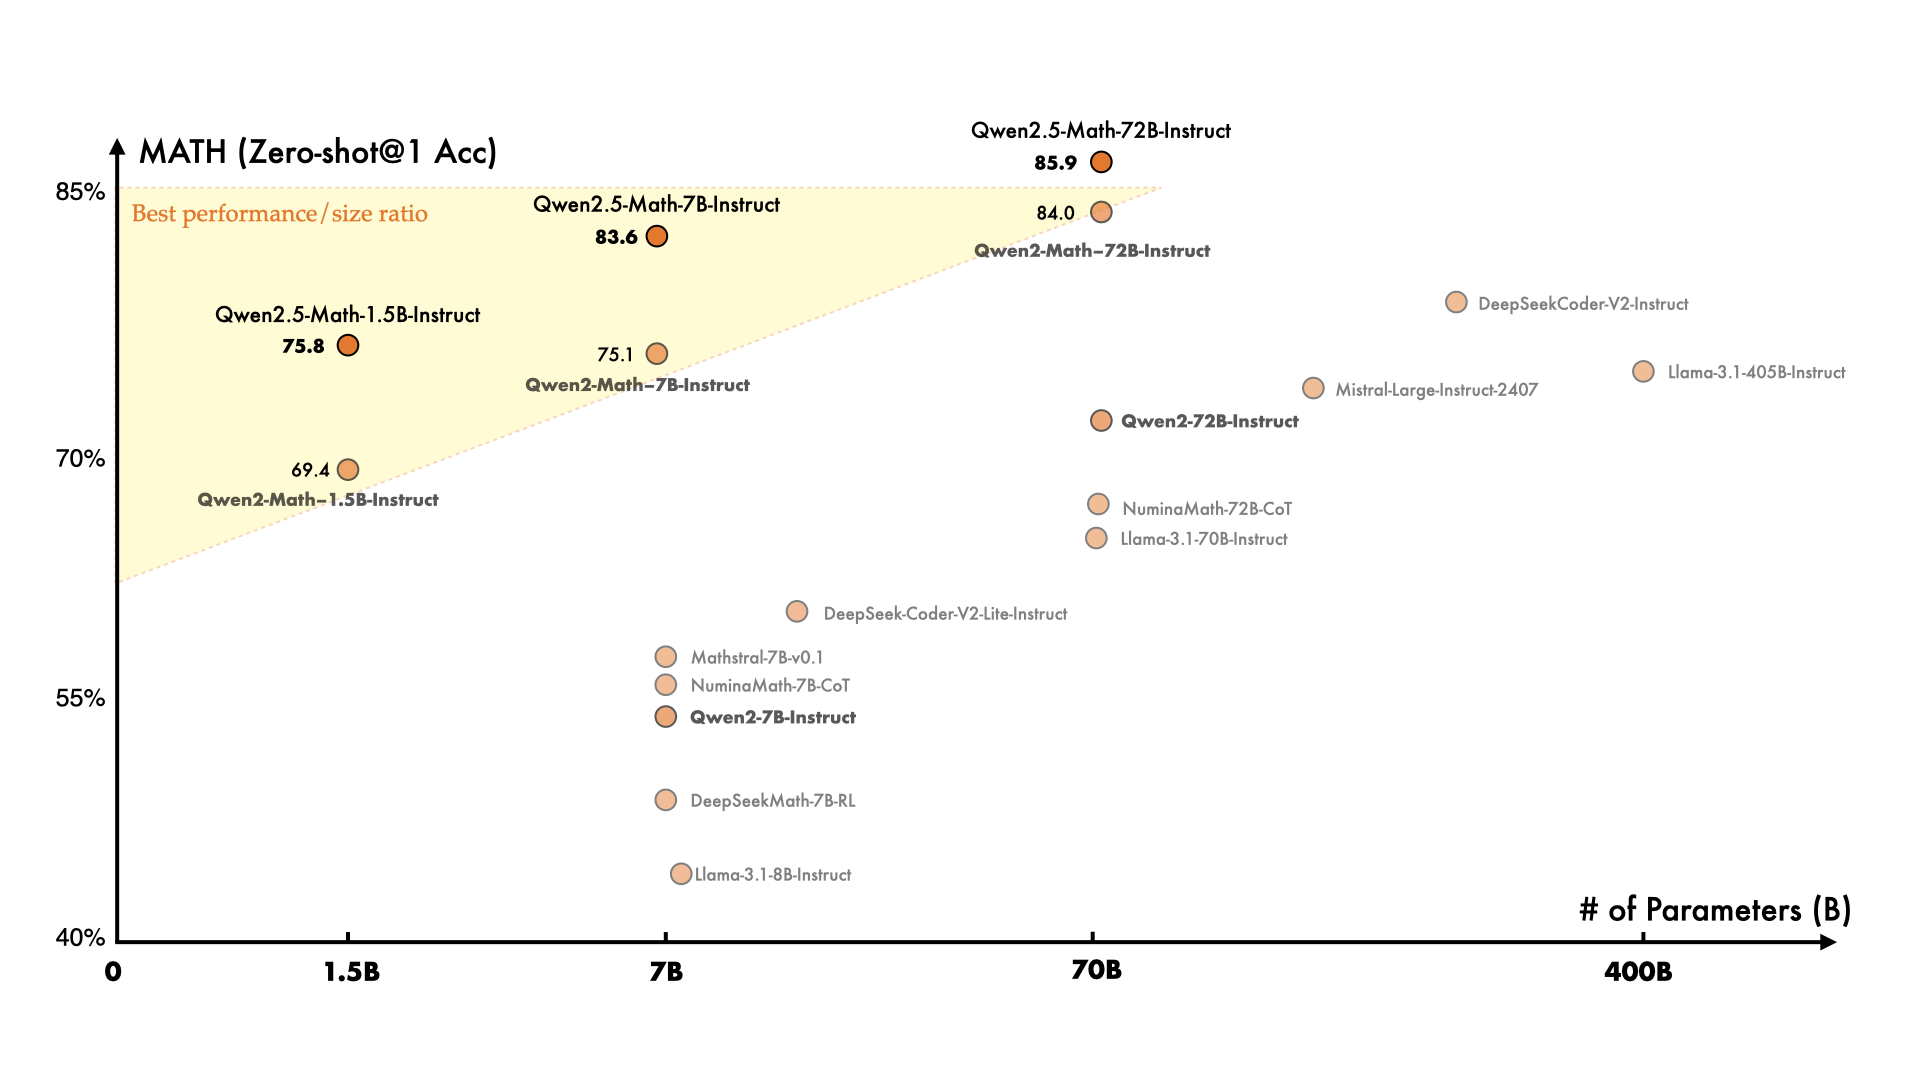
\includegraphics[width=0.8\columnwidth]{pic/all_size.png}
		\vspace{-1mm}
		\caption{The Performance of Qwen2.5-Math-1.5/7/72B-Instruct on MATH by CoT compared to models of the same size.}
		\label{fig:exp}
	\end{figure}
\end{frame}

\begin{frame}
	\begin{figure}[htbp]
		\centering
		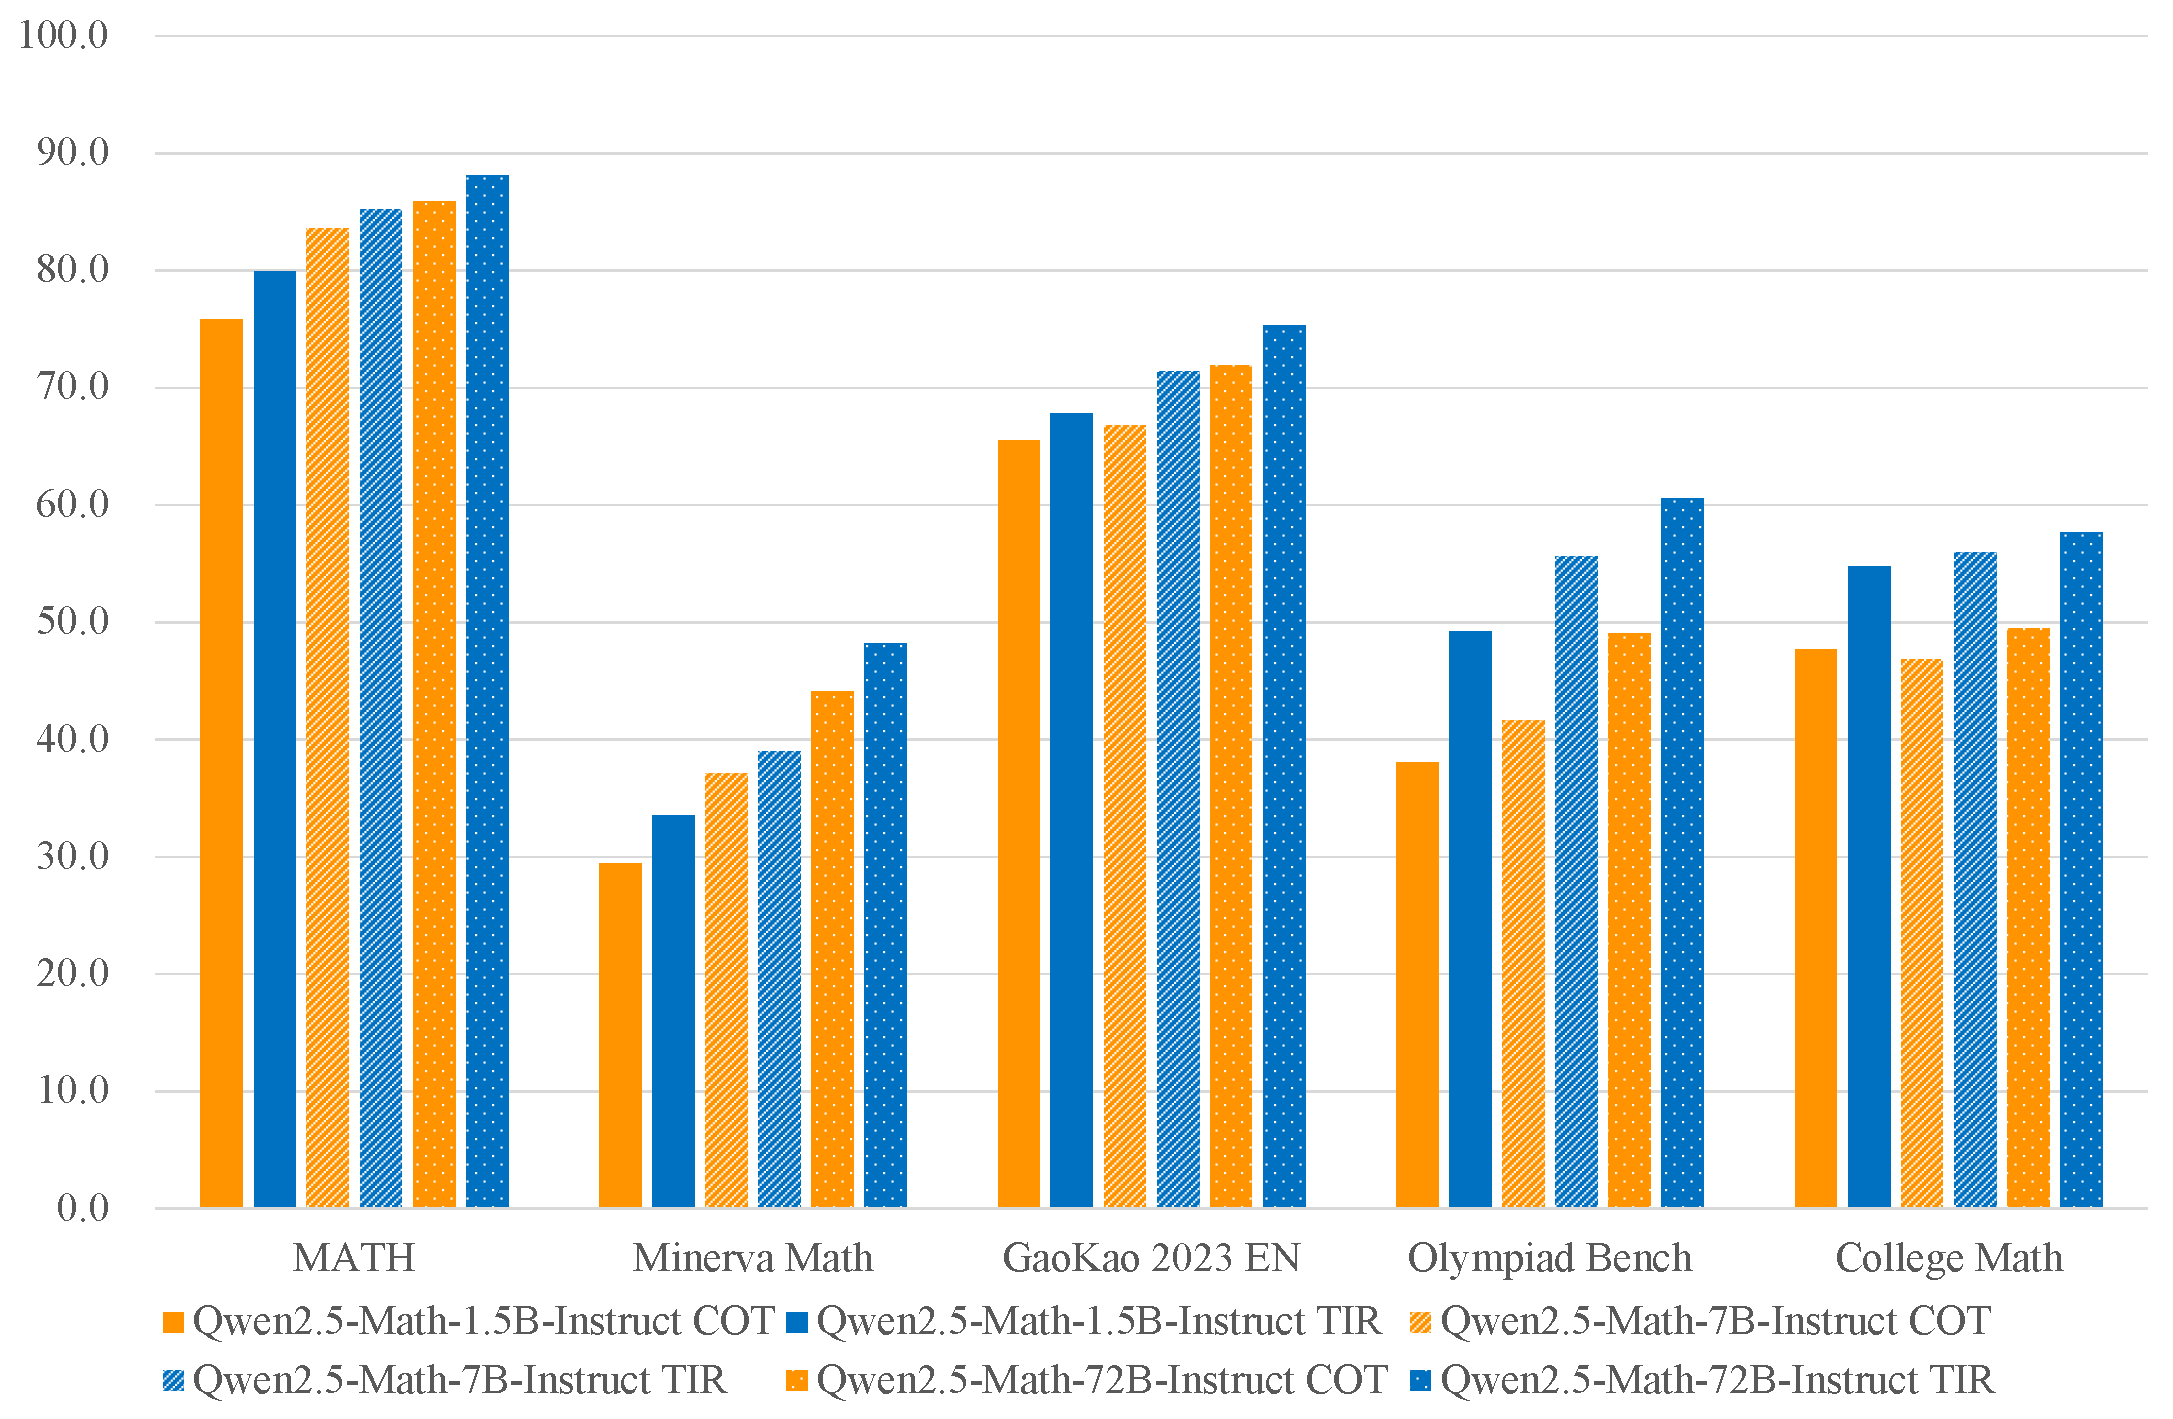
\includegraphics[width=0.7\columnwidth]{pic/COT_vs_TIR.pdf}
		% \vspace{-1mm}
		\caption{The Performance of Qwen2.5-Math-Instruct by using TIR compared to using CoT.}
		\label{fig:exp_tir}
	\end{figure}
\end{frame}
\begin{frame}
	\begin{center}
		{\Huge Thank you!}
	\end{center}
\end{frame}
% \end{frame}
